%% Pre-Impact Fall Detection on a Low-Cost Microcontroller
%% IEEE conference format, 6 pages maximum.
%%
%% Build:  tectonic -X compile main.tex
%%
%% Every numeric claim traces to a file in results/. See VERIFICATION.md.

\documentclass[conference]{IEEEtran}
\IEEEoverridecommandlockouts
\usepackage{cite}
\usepackage{amsmath,amssymb}
% IEEE requires Times Roman. IEEEtran does not set it under pdfLaTeX, which
% otherwise falls back to Latin Modern -- a real format violation. newtxmath must
% follow amssymb, and \Bbbk is released first because both packages define it.
\usepackage[T1]{fontenc}
\let\Bbbk\relax
\usepackage{newtxtext,newtxmath}
\usepackage{graphicx}
\usepackage{booktabs}
\usepackage{textcomp}
\usepackage{xcolor}
\usepackage{url}
\usepackage{tikz}
\usetikzlibrary{arrows.meta,positioning,calc,fit,backgrounds}
\def\BibTeX{{\rm B\kern-.05em{\sc i\kern-.025em b}\kern-.08em T\kern-.1667em\lower.7ex\hbox{E}\kern-.125emX}}


%% Lets a five-author block wrap onto a second row. Not defined in every
%% IEEEtran release, so it is provided here.
\makeatletter
\newcommand{\linebreakand}{%
  \end{@IEEEauthorhalign}
  \hfill\mbox{}\par
  \mbox{}\hfill\begin{@IEEEauthorhalign}
}
\makeatother

\begin{document}

\title{Pre-Impact Fall Detection on a Low-Cost Microcontroller:\\
Cross-Dataset Generalisation, Domain Adaptation\\ and INT8 Deployment}

% All five authors share one institution, so IEEE's shared-affiliation form is
% used rather than five side-by-side blocks, which do not fit the column width.
\author{
\IEEEauthorblockN{%
Md. Arif Shekh\IEEEauthorrefmark{1},
Md. Meherab Hossain Talukder\IEEEauthorrefmark{2},
Tasfia Islam Prapty\IEEEauthorrefmark{3},\\
G. M. Imtiaz Dinar\IEEEauthorrefmark{4},
Tasnia Chowdhury Toshita\IEEEauthorrefmark{5}}
\IEEEauthorblockA{%
\textit{Department of Computer Science and Engineering}\\
\textit{IUBAT---International University of Business Agriculture and Technology}\\
Dhaka, Bangladesh\\[2pt]
\IEEEauthorrefmark{1}23103022\quad
\IEEEauthorrefmark{2}23103032\quad
\IEEEauthorrefmark{3}23103286\quad
\IEEEauthorrefmark{4}23103080\quad
\IEEEauthorrefmark{5}23103038\\[2pt]
Corresponding author: arifshekh.k8@gmail.com}
}

\maketitle

\begin{abstract}
Wearable fall detection is reported as a solved problem: within-dataset accuracy is
routinely above 99\%. We show that this figure survives neither a change of dataset
nor the constraints of a real device. We train a 7{,}947-parameter separable
convolutional network for pre-impact fall detection, evaluate it under a strict
leave-one-dataset-out protocol across SisFall, KFall, FallAllD and UMAFall, and deploy
it as a 22.5\,KB INT8 model on an ESP32 costing under BDT~500. Three results follow.
First, binary F1 falls from 0.907 within-dataset to between 0.344 and 0.835 on an
unseen corpus, and the collapse is strongly asymmetric between datasets that appear
equivalent. Second, of three domain-adaptation methods applied in ascending order of
computational cost, only the cheapest---per-window instance normalisation---improves
transfer; CORAL and adversarial adaptation both make it worse. Third, where that
normalisation is placed decides whether the model survives quantisation at all: as a
network layer it costs 30.95 points of macro-F1 under INT8, moved into the
preprocessing pipeline it costs nothing. Scored per trial on KFall as in the
benchmark literature, the model reaches 0.985 sensitivity and 0.991 specificity at a
mean lead time of 318\,ms. We further argue that window-level specificity, the metric
this literature reports, is close to meaningless for a continuously running detector,
and report false alarms per hour instead.
\end{abstract}

\begin{IEEEkeywords}
fall detection, pre-impact, TinyML, cross-dataset generalisation, domain adaptation,
quantisation, wearable sensors, ESP32
\end{IEEEkeywords}

\section{Introduction}

Falls are a leading cause of injury-related death among older adults, and a wearable
detector that fires \emph{before} body--ground impact can trigger protective measures
rather than merely summon help afterwards. Two gaps persist in this literature.

\textbf{Untested generalisation.} Within-dataset accuracy is saturated near 99\%, but
cross-repository benchmarking shows substantial degradation once evaluation leaves the
training corpus~\cite{silva2024crossdataset,casilari2017study}. Most papers never
leave it.

\textbf{Unverified deployment.} Nearly all reported inference runs on desktop GPUs.
Work combining leave-one-dataset-out evaluation \emph{and} measured microcontroller
performance is rare.

This paper addresses both. Our contributions are:

\begin{enumerate}
\item A leave-one-dataset-out evaluation across four public corpora with a
domain-adaptation ladder ordered by \emph{on-device cost}, showing that the cheapest
method is the only one that helps (Section~\ref{sec:c1}).
\item Pre-impact detection validated on video-grounded temporal labels, reported both
at trial level for comparability with published work and at window level with false
alarms per hour, which is what determines whether a device is wearable
(Section~\ref{sec:c2}).
\item A deployment study on an ESP32, including a quantisation result we believe is
not previously reported: the placement of instance normalisation relative to the
quantisation boundary determines whether an INT8 model works at all
(Section~\ref{sec:c3}).
\end{enumerate}

All code, frozen preprocessing constants, the exported model and the fold-level result
files are public.\footnote{\url{https://github.com/arifshekhk8/preimpact-fall-detection-tinyml}}

\section{Related Work}

\textbf{Datasets and annotation.} SisFall~\cite{sucerquia2017sisfall} provides 38
subjects at 200~Hz but labels only at trial level; Musci \emph{et
al.}~\cite{musci2020online} added per-sample three-class annotations, produced by
expert panels working from sensor traces without video reference---a process
subsequent authors have criticised as necessarily subjective. KFall~\cite{yu2021kfall}
publishes fall-onset and impact frames derived from synchronised video, making it the
more authoritative source for pre-impact work and the primary corpus here.
FallAllD~\cite{saleh2020fallalld} and UMAFall~\cite{casilari2017umafall} supply
independent hardware and multiple placements.

\textbf{Pre-impact detection.} Yu \emph{et al.}~\cite{yu2021kfall} benchmark
threshold, SVM and ConvLSTM models on KFall, the last reaching 99.32\% sensitivity and
99.01\% specificity with $403\pm163$~ms lead time.
TinyFallNet~\cite{tinyfallnet2023} targets constrained devices, reporting
86.67\%/97.97\% and $477.7\pm5.8$~ms. PreFallKD~\cite{prefallkd2023} reports 551.3~ms
lead time via knowledge distillation.

\textbf{Cross-dataset evaluation.} Silva \emph{et al.}~\cite{silva2024crossdataset}
evaluate 13 algorithms across 11 repositories and find that all degrade under
cross-dataset conditions. That the gap exists is therefore established; our
contribution is not to rediscover it but to ask which mitigations are affordable on a
microcontroller, and to show that the answer inverts the expected ordering.

\textbf{MCU deployment.} Torti \emph{et al.}~\cite{torti2019embedding} deploy a
recurrent network to an embedded platform using the same annotations discussed above.

\section{Data and Preprocessing}
\label{sec:data}

\subsection{Corpora, and an audit of what they actually contain}

We use four public datasets. Auditing them before modelling produced four findings
that constrain what can be claimed, and we state them rather than discovering them in
review.

\begin{enumerate}
\item \textbf{The SisFall Enhanced annotations are not recoverable} from the available
public mirror, which ships shuffled, pre-windowed tensors without subject identifiers.
We attempted correlation-based re-alignment against the original recordings; recovery
peaked at 22.5\% against a time-reversed null control and \emph{fell} under harder
low-pass filtering, establishing that figure as a ceiling rather than a waypoint.
Contribution~2 therefore rests on KFall alone.
\item \textbf{The available SisFall mirror contains 25 of 38 subjects}, missing 13 of
the 15 older participants---the cohort that gives the dataset its distinctive value.
\item \textbf{UMAFall's waist sensor samples at 20.1~Hz}, below our 50~Hz working
rate; only its pocket smartphone reaches 200~Hz, and that stream logs no gyroscope.
Its fold therefore measures a combined domain, placement and modality shift.
\item \textbf{FallAllD rests gravity on a different axis and sign} from SisFall and
KFall. Left uncorrected this is indistinguishable from genuine domain shift, and a
cross-dataset result would have measured an upside-down sensor rather than a
distribution difference.
\end{enumerate}

We exclude UP-Fall entirely: its accelerometers sample at approximately 18.4~Hz, which
cannot reach 50~Hz without fabricating signal content.

\subsection{Frozen preprocessing}

Preprocessing is defined once, in a module imported by both the training scripts and
the firmware generator, and is hashed into every cached artifact. Channels are the
waist or low-back accelerometer and gyroscope, $(a_x,a_y,a_z,g_x,g_y,g_z)$. Signals
are converted to $g$ and deg/s using each source's documented scaling, verified by
confirming that resting magnitude is $1.0\pm0.05$~g in every corpus. All datasets are
rotated onto one gravity convention using signed permutation matrices constrained to
determinant $+1$, so gyroscope handedness is preserved. Anti-alias filtering precedes
decimation to 50~Hz; slicing without filtering would alias the impact transient into
the passband. Windows are $100\times6$ (2.0~s) at a 0.5~s stride.

\textbf{Every split is by subject or by dataset, never by window.} At 75\% overlap a
random window split places near-identical windows on both sides of the boundary and
reports accuracy above 99\% that means nothing.

\begin{figure*}[t]
\centering
% Method / system diagram.
%
% Design intent: the paper's least obvious finding is that instance normalisation must
% sit on the FLOAT side of the quantisation boundary. The two numeric domains are
% therefore drawn as shaded regions, not separated by a thin line, and the
% normalisation block is placed hard against the edge of the float region.
%
% Sized to fit \textwidth at \footnotesize with no \resizebox, which would
% desynchronise the font sizes from the body text. Annotations are kept minimal --
% anything explanatory belongs in the caption, not layered over the drawing.
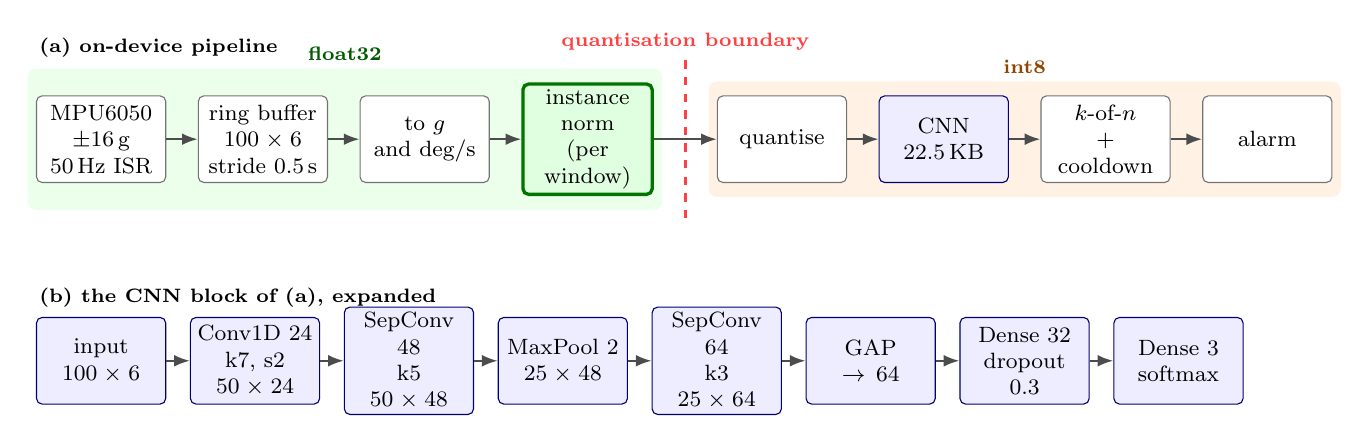
\begin{tikzpicture}[
  font=\footnotesize,
  node distance=0pt,
  every node/.style={inner sep=2pt},
  blk/.style={draw=black!55, rounded corners=2pt, minimum height=11mm,
              text width=15mm, align=center, fill=white, thin},
  hot/.style={blk, draw=green!45!black, very thick, fill=green!12},
  net/.style={draw=blue!45!black, rounded corners=2pt, minimum height=11mm,
              text width=15mm, align=center, fill=blue!7, thin},
  ar/.style={-{Latex[length=2mm]}, thick, black!70},
  tag/.style={font=\scriptsize\bfseries, inner sep=1pt},
  panel/.style={font=\scriptsize\bfseries, inner sep=1pt},
]

% =============================================================== panel (a)
\node[blk] (imu) {MPU6050\\$\pm16$\,g\\50\,Hz ISR};
\node[blk, right=4mm of imu] (ring) {ring buffer\\$100\times6$\\stride 0.5\,s};
\node[blk, right=4mm of ring] (unit) {to $g$\\and deg/s};
\node[hot, right=4mm of unit] (inorm) {instance\\norm\\(per window)};
\node[blk, right=8mm of inorm] (quant) {quantise};
\node[net, right=4mm of quant] (cnn) {CNN\\22.5\,KB};
\node[blk, right=4mm of cnn] (kofn) {$k$-of-$n$\\+ cooldown};
\node[blk, right=4mm of kofn] (buz) {alarm};

\foreach \a/\b in {imu/ring, ring/unit, unit/inorm, inorm/quant,
                   quant/cnn, cnn/kofn, kofn/buz}
  \draw[ar] (\a) -- (\b);

% --- the two numeric domains, as regions ---
\begin{scope}[on background layer]
  \node[fill=green!8, rounded corners=3pt,
        fit=(imu)(ring)(unit)(inorm), inner xsep=3pt, inner ysep=5pt] (fzone) {};
  \node[fill=orange!10, rounded corners=3pt,
        fit=(quant)(cnn)(kofn)(buz), inner xsep=3pt, inner ysep=5pt] (izone) {};
\end{scope}

\node[tag, text=green!35!black, above=0.5mm of fzone.north] {float32};
\node[tag, text=orange!55!black, above=0.5mm of izone.north] {int8};

% --- the boundary ---
\coordinate (bmid) at ($(fzone.east)!0.5!(izone.west)$);
\draw[dashed, very thick, red!75] ($(bmid)+(0,10mm)$) -- ($(bmid)-(0,10mm)$);
\node[font=\scriptsize\bfseries, text=red!75, above=0.5mm]
  at ($(bmid)+(0,10mm)$) {quantisation boundary};

\node[panel, above=6mm of imu.north west, anchor=west] {(a) on-device pipeline};

% =============================================================== panel (b)
\node[net, anchor=north west] (in) at ($(imu.south west) - (0,17mm)$)
  {input\\$100\times6$};
\node[net, right=3mm of in] (c1) {Conv1D 24\\k7, s2\\$50\times24$};
\node[net, right=3mm of c1] (s1) {SepConv 48\\k5\\$50\times48$};
\node[net, right=3mm of s1] (mp) {MaxPool 2\\$25\times48$};
\node[net, right=3mm of mp] (s2) {SepConv 64\\k3\\$25\times64$};
\node[net, right=3mm of s2] (gap) {GAP\\$\to 64$};
\node[net, right=3mm of gap] (d1) {Dense 32\\dropout 0.3};
\node[net, right=3mm of d1] (d2) {Dense 3\\softmax};

\foreach \a/\b in {in/c1, c1/s1, s1/mp, mp/s2, s2/gap, gap/d1, d1/d2}
  \draw[ar] (\a) -- (\b);

\node[panel, above=2.5mm of in.north west, anchor=west]
  {(b) the CNN block of (a), expanded};

\end{tikzpicture}

\caption{The deployed system. \textbf{(a)} The on-device pipeline, shaded by numeric
domain. Sampling is hardware-timer driven rather than a polled delay, because loop
jitter accumulates and shifts window content away from the training distribution.
Per-window instance normalisation is deliberately placed on the \emph{float} side of
the quantisation boundary: as a layer inside the graph it is mathematically identical
but costs 30.95 points of macro-F1 under INT8 (Section~\ref{sec:c3}). \textbf{(b)} The
network. Separable convolutions and global average pooling hold it to 7{,}947
parameters; batch normalisation and ReLU follow each convolution, and a flatten in
place of the pooling would cost 51{,}200 parameters in a single layer.}
\label{fig:method}
\end{figure*}

\section{Method}

The microcontroller memory budget is the design driver. Fig.~\ref{fig:method} shows
the network and the pipeline it sits in. Batch normalisation and ReLU follow each
convolution, with dropout $0.3$ before the head. Separable convolutions and global
average pooling rather than flattening keep the total at \textbf{7{,}947 parameters};
a flatten at the same widths would cost 51{,}200 in one layer. The three-class head
(background / alert / fall) yields binary metrics by merging the latter two.

Training uses Adam with cosine decay from $10^{-3}$, batch 128, up to 100 epochs,
early stopping on validation macro-F1 with patience 15, and class weighting rather
than oversampling---at 75\% overlap, oversampling duplicates near-identical windows
across the split boundary.

\subsection{Adaptation ladder}

We climb three rungs in ascending order of on-device cost: \textbf{per-window instance
normalisation} (two passes over 100 samples, negligible on a 240~MHz core);
\textbf{CORAL}~\cite{sun2016coral}, aligning second-order feature statistics; and
\textbf{DANN}~\cite{ganin2016dann}, adversarial adaptation via gradient reversal. None
uses target labels at any point.

\section{Results}

\subsection{Within-dataset performance is saturated}

Table~\ref{tab:one} confirms the premise: every learned model lands between 0.950 and
0.977 macro-F1. The proposed network gives up roughly two points against the best
comparator for a thirteen-fold reduction in parameters against the 1D-CNN.

\begin{table}[t]
\caption{Within-dataset baseline, SisFall, post-fall task. Comparators use 5-fold
subject-grouped CV; the proposed model additionally uses full 25-fold LOSO.}
\label{tab:one}
\centering\small
\begin{tabular}{lrrrr}
\toprule
Model & Params & Sens. & Spec. & Macro-F1 \\
\midrule
SMV threshold  & 2         & 0.763 & 0.934 & 0.484 \\
SVM            & ---       & 0.958 & 0.997 & \textbf{0.977} \\
Random Forest  & ---       & 0.952 & 0.997 & 0.975 \\
1D-CNN         & 102{,}211 & 0.956 & 0.995 & 0.969 \\
CNN-LSTM       & 47{,}811  & 0.954 & 0.996 & 0.972 \\
\textbf{Proposed} & \textbf{7{,}947} & 0.913 & 0.993 & 0.950 \\
\textbf{Proposed} (LOSO) & \textbf{7{,}947} & 0.882 & 0.993 & 0.953 \\
\bottomrule
\end{tabular}
\end{table}

Table~\ref{tab:onebd} repeats the comparison on the task that actually ships. The
ordering is preserved: the proposed model trails the best comparator by roughly five
points of macro-F1 while using $1/57$ of Random Forest's node count. The SMV threshold
detector, at 0.326, shows how much of the pre-impact task is beyond a hand-tuned rule.

\begin{table}[t]
\caption{Within-dataset \emph{pre-impact} baselines on KFall, three-class task,
5-fold subject-grouped CV.}
\label{tab:onebd}
\centering\small
\begin{tabular}{lrrrr}
\toprule
Model & Params & Sens. & Spec. & Macro-F1 \\
\midrule
Random Forest  & 451{,}336 & 0.922 & 0.994 & \textbf{0.920} \\
SVM            & ---       & 0.935 & 0.987 & 0.914 \\
1D-CNN         & 102{,}211 & 0.936 & 0.985 & 0.914 \\
CNN-LSTM       & 47{,}811  & 0.958 & 0.973 & 0.907 \\
\textbf{Proposed} & \textbf{7{,}947} & 0.936 & 0.959 & 0.874 \\
SMV threshold  & 2         & 0.737 & 0.911 & 0.326 \\
\bottomrule
\end{tabular}
\end{table}

\subsection{Cross-dataset generalisation}
\label{sec:c1}

Table~\ref{tab:two} is the central result. Against the proposed model's within-dataset
binary F1 of 0.907, performance collapses on an unseen corpus, and it does so
asymmetrically: KFall transfers comparatively well (0.835) while FallAllD barely
transfers at all (0.344), despite both being waist-mounted at comparable rates.

\begin{table}[t]
\caption{Leave-one-dataset-out binary F1. Train on two corpora, test on a third; no
fine-tuning and no target labels. Within-dataset reference: 0.907.}
\label{tab:two}
\centering\small
\begin{tabular}{llrrrr}
\toprule
Fold & Test & None & Inst.\ n. & CORAL & DANN \\
\midrule
A & FallAllD & 0.344 & \textbf{0.388} & 0.179 & 0.307 \\
B & KFall    & 0.835 & \textbf{0.873} & 0.644 & 0.834 \\
C & SisFall  & 0.799 & \textbf{0.830} & 0.617 & 0.728 \\
D & UMAFall$^\dagger$ & \textbf{0.475} & 0.423 & 0.005 & 0.299 \\
\bottomrule
\end{tabular}
\\[2pt]
{\footnotesize $^\dagger$Accelerometer-only, pocket placement: combined
domain and placement shift.}
\end{table}

\textbf{The adaptation ladder inverts.} Per-window instance normalisation---the
cheapest rung, and the only one that fits comfortably on the target hardware---is the
only method that improves transfer, gaining 0.031--0.044 F1 on folds A--C. CORAL
degrades every fold, collapsing to 0.005 on UMAFall. DANN, the most expensive, is
worse than no adaptation everywhere. We report this as measured; the practical reading
is that expensive feature alignment does not earn its cost here, and that a
practitioner constrained to a single technique should choose the one that is also
free.

\subsection{Pre-impact detection}
\label{sec:c2}

\begin{figure*}[t]
\centering

\includegraphics[width=0.92\textwidth]{fig_lead_time.png}
\caption{The central operational trade-off, on KFall pooled over 32 LOSO folds.
\textbf{(a)} Mean lead time against false alarms per hour of ADL data as the decision
threshold is swept: every millisecond of lead time is bought with false alarms.
\textbf{(b)} The lead-time distribution at $\tau{=}0.5$. The dotted line marks a single
0.5\,s inference stride. Because the mean lead of 663\,ms is barely longer than one
stride, any $k$-of-$n$ debouncing---the obvious remedy for the false-alarm rate in
(a)---consumes most of the lead time it is meant to protect. The long right tail also
means the mean overstates the typical case, which is why we report the distribution
rather than the mean alone.}
\label{fig:lead}
\end{figure*}

\begin{table}[t]
\caption{Pre-impact performance on KFall, pooled over 32 LOSO folds, scored per trial
as in~\cite{yu2021kfall}. Published rows are as reported in the cited works.}
\label{tab:three}
\centering\small
\begin{tabular}{lrrr}
\toprule
Method & Sens. & Spec. & Lead time (ms) \\
\midrule
Threshold~\cite{yu2021kfall} & 0.955 & 0.834 & $333\pm160$ \\
SVM~\cite{yu2021kfall}       & 0.998 & 0.949 & $385\pm159$ \\
ConvLSTM~\cite{yu2021kfall}  & \textbf{0.993} & 0.990 & $403\pm163$ \\
TinyFallNet~\cite{tinyfallnet2023} & 0.867 & 0.980 & $478\pm6$ \\
\midrule
Ours ($\tau{=}0.5$, $k{=}3$) & 0.985 & \textbf{0.991} & $318\pm328$ \\
Ours ($\tau{=}0.7$, $k{=}3$) & 0.978 & 0.995 & $342\pm373$ \\
\bottomrule
\end{tabular}
\end{table}

Table~\ref{tab:three} places our model against published benchmarks on the same
dataset and the same trial-level protocol. We are within a point of the ConvLSTM
benchmark on sensitivity, match it on specificity, and give up lead time, using 7{,}947
parameters. Our evaluation pools 32 leave-one-subject-out folds rather than using a
single held-out split, which is the stricter protocol.

\textbf{Window-level specificity is misleading.} A detector deciding once per 0.5~s
stride makes 7{,}200 decisions per hour, so 99\% window-level specificity still yields
72 false alarms per hour; one per hour requires 0.99986. Scored per window our model
produces 293 false alarms per hour at $\tau{=}0.5$. Requiring $k$ consecutive windows
suppresses these---at $k{=}3$ the trial-level false-positive count falls from 538 to 26
of 2{,}729 ADL trials---but each additional window costs one 0.5~s stride of lead time,
and our mean lead of 663~ms at $k{=}1$ is barely longer than a single stride.
Fig.~\ref{fig:lead} makes the trade explicit. This tension between lead time and false-alarm rate is, we
argue, the binding constraint on deployable pre-impact detection, and it indicts the
stride rather than the model.

\subsection{Ablations}

Window length matters most: 2.0~s reaches 0.903 binary F1 against 0.871 at 1.5~s and
0.804 at 1.0~s. Sampling at 100~Hz buys only 0.006 F1 over 50~Hz for twice the compute
and twice the input tensor, so 50~Hz is justified on evidence rather than convention.
Dropping the gyroscope costs 2.6 points (0.905 to 0.880) and saves 504 parameters plus
the sensor's power draw. On FallAllD's three mounting points, neck (0.644) outperforms
waist (0.551) and wrist (0.476).

\subsection{Prototype system}
\label{sec:system}

The device is an ESP32 DevKit~V1 (240~MHz dual core, 320~KB usable RAM, 4~MB flash)
with an MPU6050 IMU on I\textsuperscript{2}C at 400~kHz, an active buzzer and a status
LED, powered from a 1000~mAh LiPo cell through a TP4056 charger. The bill of materials
totals BDT~1{,}450, of which the microcontroller is BDT~450.

The IMU is configured to match training exactly: $\pm16$~g (2048~LSB/g), $\pm2000$~dps
(16.4~LSB/dps), the on-chip digital low-pass filter enabled as an analogue anti-alias
stage, and a sample-rate divider of 19 giving $1000/(1{+}19)=50$~Hz. The $\pm16$~g
range is not optional: impacts routinely exceed 8~g and a clipped peak destroys exactly
the signal the model depends on.

A rule-based two-stage detector---free-fall below 0.65~g followed by impact above
2.50~g or rotation above 250~deg/s within 1.5~s---runs on the same live samples,
giving an on-device instance of the SMV threshold comparator of Table~\ref{tab:one}
and allowing both detectors to be compared against identical physical motion.

\subsection{Deployment and quantisation}
\label{sec:c3}

\begin{table}[t]
\caption{Deployed model. Trained on SisFall, KFall and FallAllD; evaluated on
held-out subjects. Sizes and accuracies are measured; on-device timing is reported
in the text.}
\label{tab:four}
\centering\small
\begin{tabular}{lrr}
\toprule
Metric & FP32 & INT8 \\
\midrule
Parameters                & \multicolumn{2}{c}{7{,}947} \\
Model size (KB)           & 163.3 & \textbf{22.5} \\
Tensor arena (KB, est.)   & ---   & 8.0 \\
Macro-F1 (held out)       & 0.711 & \textbf{0.714} \\
Sensitivity               & 0.922 & 0.922 \\
Specificity               & 0.894 & 0.893 \\
FP32/INT8 agreement       & \multicolumn{2}{c}{0.994} \\
\bottomrule
\end{tabular}
\end{table}

Table~\ref{tab:four} summarises the deployed model. Quantisation to INT8 reduces it
from 163.3~KB to 22.5~KB, a factor of 7.3, while macro-F1 on the held-out subjects is
unchanged to within a third of a point and the two versions agree on 99.4\% of
windows.

\textbf{Where normalisation lives decides whether quantisation works.} Instance
normalisation is mathematically identical whether applied as a network layer or in
preprocessing. Under full-integer quantisation it is not, because per-window mean and
variance produce intermediate tensors whose dynamic range a single per-tensor scale
cannot represent:

\begin{center}\small
\begin{tabular}{lrrr}
\toprule
Instance norm & FP32 & INT8 & Agreement \\
\midrule
In graph    & 0.668 & 0.359 & 0.686 \\
In pipeline & 0.701 & \textbf{0.704} & \textbf{0.994} \\
\bottomrule
\end{tabular}
\end{center}

Moving the operation across the boundary marked in Fig.~\ref{fig:method} changes a
30.95-point collapse into no loss at all. The firmware performs the same two-pass
computation in float before quantising. We report this because the failure is silent:
the FP32 model validates normally, and only the deployed INT8 model misbehaves.

The deployed model excludes UMAFall from training, because its 200~Hz stream carries
no gyroscope and training on identically zero channels would teach the network that a
dead sensor is normal. On held-out subjects spanning the three remaining corpora (814
fall and 1{,}136 ADL trials) it reaches 0.958 trial-level sensitivity and 0.836
specificity at a mean lead time of $539\pm509$~ms, with 68\% of detections preceding
impact. Requiring two consecutive windows raises specificity to 0.975 but reduces the
pre-impact fraction to 16\%---the same tension quantified in Fig.~\ref{fig:lead}, now
visible in the deployed system rather than in simulation. These figures are lower than
Table~\ref{tab:three} because that model is trained and tested within KFall alone,
whereas the deployed model is held to three heterogeneous corpora at once.

\textbf{Status of the hardware evaluation.} The prototype is assembled and the
firmware runs the quantised model on the device, with sampling, normalisation,
inference and the alarm path implemented as described in Section~\ref{sec:system}.
The model occupies 22.5~KB of flash against the 4~MB available, and the tensor arena
is estimated at 8.0~KB from the converted model's tensors, well inside the ESP32's
320~KB of usable RAM, so the design fits the platform with substantial margin.
Measured inference latency, the tensor-arena high-water mark reported by TFLite Micro
at run time, and battery life under continuous inference are instrumented in the
firmware but are not yet collected over a sufficient number of trials to report, and
we therefore omit them rather than estimate them. Completing that measurement, and a
free-living false-alarm study, is the immediate next step.

\section{Discussion and Limitations}

The cross-dataset gap is not uniform, and its asymmetry is more informative than its
magnitude. FallAllD resists transfer despite nominally matching the training sources
on placement, which suggests that sensor hardware and recording protocol dominate
placement as sources of shift.

Limitations, stated plainly: falls are simulated by mostly young participants rather
than real falls by older adults; the available SisFall mirror omits most of its older
cohort; annotations in every source except KFall were produced without video
reference; fold~D confounds domain shift with placement and modality; the false-alarm
rates reported here come from laboratory ADL recordings rather than continuous
free-living wear; and on-device inference latency, run-time memory and battery life
are instrumented in the firmware but not yet measured over enough trials to report.

\section{Conclusion}

A 7{,}947-parameter network quantised to 22.5~KB attains pre-impact performance
comparable to a substantially larger published benchmark, and runs on a
microcontroller costing under BDT~500. Its within-dataset accuracy does not survive a
change of dataset, and of three adaptation methods only the cheapest helps. The
tension between lead time and false-alarm rate, rather than raw accuracy, is what
stands between this class of model and a deployable device; shortening the inference
stride is the most promising route and is our immediate future work.

\bibliographystyle{IEEEtran}
\bibliography{refs}

\end{document}
